% !TEX TS-program = pdflatexmk
%header and footer for separate chapter files

\ifx\whole\undefined
\documentclass[12pt, leqno]{book}
\usepackage{graphicx}
\input style-for-curves.sty
\usepackage{hyperref}
\usepackage{showkeys} %This shows the labels.
%\usepackage{SLAG,msribib,local}
%\usepackage{amsmath,amscd,amsthm,amssymb,amsxtra,latexsym,epsfig,epic,graphics}
%\usepackage[matrix,arrow,curve]{xy}
%\usepackage{graphicx}
%\usepackage{diagrams}
%
%%\usepackage{amsrefs}
%%%%%%%%%%%%%%%%%%%%%%%%%%%%%%%%%%%%%%%%%%
%%\textwidth16cm
%%\textheight20cm
%%\topmargin-2cm
%\oddsidemargin.8cm
%\evensidemargin1cm
%
%%%%%%Definitions
%\input preamble.tex
%\input style-for-curves.sty
%\def\TU{{\bf U}}
%\def\AA{{\mathbb A}}
%\def\BB{{\mathbb B}}
%\def\CC{{\mathbb C}}
%\def\QQ{{\mathbb Q}}
%\def\RR{{\mathbb R}}
%\def\facet{{\bf facet}}
%\def\image{{\rm image}}
%\def\cE{{\cal E}}
%\def\cF{{\cal F}}
%\def\cG{{\cal G}}
%\def\cH{{\cal H}}
%\def\cHom{{{\cal H}om}}
%\def\h{{\rm h}}
% \def\bs{{Boij-S\"oderberg{} }}
%
%\makeatletter
%\def\Ddots{\mathinner{\mkern1mu\raise\p@
%\vbox{\kern7\p@\hbox{.}}\mkern2mu
%\raise4\p@\hbox{.}\mkern2mu\raise7\p@\hbox{.}\mkern1mu}}
%\makeatother

%%
%\pagestyle{myheadings}

%\input style-for-curves.tex
%\documentclass{cambridge7A}
%\usepackage{hatcher_revised} 
%\usepackage{3264}
   
\errorcontextlines=1000
%\usepackage{makeidx}
\let\see\relax
\usepackage{makeidx}
\makeindex
% \index{word} in the doc; \index{variety!algebraic} gives variety, algebraic
% PUT a % after each \index{***}

\overfullrule=5pt
\catcode`\@\active
\def@{\mskip1.5mu} %produce a small space in math with an @

\title{Personalities of Curves}
\author{\copyright David Eisenbud and Joe Harris}
%%\includeonly{%
%0-intro,01-ChowRingDogma,02-FirstExamples,03-Grassmannians,04-GeneralGrassmannians
%,05-VectorBundlesAndChernClasses,06-LinesOnHypersurfaces,07-SingularElementsOfLinearSeries,
%08-ParameterSpaces,
%bib
%}

\date{\today}
%%\date{}
%\title{Curves}
%%{\normalsize ***Preliminary Version***}} 
%\author{David Eisenbud and Joe Harris }
%
%\begin{document}

\begin{document}
\maketitle

\pagenumbering{roman}
\setcounter{page}{5}
%\begin{5}
%\end{5}
\pagenumbering{arabic}
\tableofcontents
\fi


\chapter{Rational Normal Scrolls}
\label{ScrollsChapter}

\begin{verbatim}
 The naming of cats is a difficult matter,
 It isn't just one of your everyday games.
 You may think that I am as mad as a hatter,
 When I tell you each cat must have three different names.
 The first is the name that the family use daily ...
 But I tell you, a cat needs a name that's particular ...
 But above and beyond there's still one name left over,  ...
 [his] deep and inscrutable, singular name.

 
 --T.S.Eliot, Practical Cats
\end{verbatim}

\fix{Notation in this chapter the field often has to be algebraically closed. I am writing it as $\CC$,
but this will be easy to replace globally with $k$ if this seems desirable -- in which case we should add a blanket assumption. Also we write
$\PP$ instead of $\PP_{\CC}$.}

Some of the simplest subvarieties in projective space are the \emph{rational normal scrolls}. They appear in many contexts in algebraic geometry, and are useful for describing the embeddings of curves of low degree and genus. 

We begin this chapter by giving three different characterizations of these varieties, each useful in a different context: First a classical geometric construction that gives a good picture, then an algebraic description that allows one to ``find" the scrolls containing a given variety, and then a more modern geometric definition that makes it easy to understand the divisors on a scroll. Finally, we turn to some of the applications to the embeddings of curves.

In each section we will focus on the 2-dimensional case, both because this is the case that occurs in our applications, and to simplify the discussion. We will also indicate the surprisingly simple extension to higher dimensions.

In this chapter we will refer to rational normal scrolls simply as scrolls. The third characterization we will give lends itself to a natural generalization to families of irrational ruled varieties, which we'll briefly mention, and the reader should be aware that in the literature the word ``scroll'' is used for this wider class.

[Notation:  $\PP^{N}$ and $\PP^{1}$ mean $\PP_{\CC}^{N}$ and $\PP_{\CC}^{1}$. ]

\section{Some classical geometry (the name the family use daily)}\label{daily name}

Recall that the image of the map 
$$
\PP^1\to\PP^a: (s,t) \mapsto (s^a, s^{a-1}t, \dots, t^a),
$$
corresponding to the complete linear series
$|\cO_{\PP^1}(a)|$, is called a \emph{rational normal curve}; it is, up to linear transformations, the unique nondegenerate curve of degree $a$ in $\PP^a$ (\ref{*****}).\fix{this must have been done in an early chapter!}

Scrolls are one answer to the question: ``What are the higher-dimensional analogues of rational normal curves?'' To construct a scroll of dimension 2, we choose integers $0<a_1, a_2$ and consider  a projective space 
$$
\PP^{a_1+a_2+1} = \PP_B(\CC^{a_1+1}\oplus \CC^{a_2+1})
$$
with its two subspaces $\PP^{a_i} = \PP_B(\CC^{a_i+1})$. We choose rational normal curves $C_i\subset \PP^{a_i}$, and we choose an isomorphism $\phi: C_1\to C_2$. We define the scroll $S(a_1, a_2)$ to be the union of the lines
$$
S(a_1,a_2) := \bigcup_{p\in C_1} \overline{p, \phi(p)}.
$$
We call the curves $C_{a_{1}}$ and $C_{a_{2}}$ the \emph{directrices} (singular: directrix) of the scroll, and we call the lines $\overline{p, \phi(p)}$ the \emph{rulings} of the scroll.

It is not hard to prove directly that $S(a_1,a_2)$ is an algebraic variety, and we shall soon write down its defining equations.

From this description we can immediately deduce the dimension and degree of the scroll:
\begin{proposition}
\begin{enumerate}
\item $S(a_1,a_2)$ is a nondegenerate surface.
 \item $S(a_1,a_2)$ has degree $a_1+a_2$, and codimension $a_1+a_2-1.$
 \end{enumerate}

\end{proposition}\label{deg and codim}
\begin{proof}
 The rational normal curves separately span the spaces $\PP^{a_i}$, so a hyperplane containing both of them would contain $\overline{\PP^{a_1}, \PP^{a_{2}+1}} = \PP$, proving nondegeneracy. 
 
 It is clear from our description that $S$ is 2-dimensional, and thus of
codimension $a_{1}+a_{2}+1 -2 = a_{1}+a_{2}-1$. 

To compute the degree, we choose a general hyperplane $H$ containing $\PP^{a_{1}}$. The intersection $H\cap C_{2}$ consists of $a_{2}$ reduced points. Thus the intersection $H\cap S$ consists of $C_{1}$ and the $a_{2}$ reduced lines connecting 
the points of $H\cap C_{2}$ with their corresponding points on $C_{1}$; this union has degree $a_{1}+a_{2}$.
\end{proof}

A completely parallel construction creates rational normal scrolls of dimension $r$. Set $N = \sum_{i=1}^{r}(a_{i}+1)$, where each $a_{i}>0$ and
decompose $\CC^{N}$ as
$$
\CC^{\sum_{i=1}^{r}(a_{i}+1)} = \oplus_{i=1}^{r}\CC^{a_{i}+1}.
$$
Let $\PP^{a_{i}}\subset \PP^{N}$ be the subspaces corresponding to the summands,  choose
rational normal curves $C_{i}\subset \PP^{a_{i}}$ and choose isomorphisms $C_{1}\to C_{i}$. 
Set
$$
S:=S(a_{1}, \dots, a_{r}) = \bigcup_{p\in C_{1}}\overline{p, \phi_{2}(p), \dots, \phi_{r}(p)}.
$$
The variety $S$ is nondegenerate of codimension $N-r$ and degree $\sum_{i}a_{i} = N-r+1$. The proof is similar to the one we gave for $r=2$.
Note the case $r=1$, in which $S(a)$ is simply the rational normal curve of degree $a$. 

To put this result in context, we recall an elementary fact of projective geometry:
 
\begin{proposition}\label{minimal degree}
 Any nondegenerate variety of codimension $c$ in $\PP^{N}$ has degree $\geq c +1$.
\end{proposition}

\begin{proof} We do induction on $c$.The case $c=0$ being trivial,
 we may assume that $c\geq1$. A general plane $L\subset \PP^{N}$ meets $X$ in $\deg X$
 distinct general points, which must be nonsingular points of $X$.
 
Let $p\in L\cap X$ be a point. If every secant to $X$ through $p$ lies entirely in $X$, then $X$ is a cone over $p$; but since $p$ was a general point, this would imply that $X$ is a plane, contradicting non-degeneracy. 

It follows that the projection $\pi_{p}:X \to \PP^{N-1}$ is a generically finite (rational) map from $X$ to $X' := \pi_{p}(X)$,
and thus $\dim X' = \dim X$ and $\codim X' = \codim X+1$. The plane 
$\pi_{p}(L)$ meets $X'$ in the images of the points of $L\cap X$ other than $p$, so
$\deg X\geq \deg X'+1$. By induction, $\deg X' \geq \codim X'+1 = \codim X$, completing the argument.
\end{proof}

Thus scrolls are \emph{varieties of minimal degree}. The reader already knows that the rational normal curves of degree $a$ in $\PP^{a}$ are the only curves of degree $a$ and codimension $a-1$. A celebrated Theorem of Del Pezzo (for surfaces) and Bertini (in general) generalizes this statement:

\begin{theorem}\label{classification of scrolls} 
Any nondegenerate variety $X\subset \PP^{N}$ with with $\deg X = \codim X+1$, is either a scroll or the Veronese surface in $\PP^{5}$ or a cone over one of these.
\end{theorem}

A proof is given in the appendix to this chapter.

One interesting way to view the construction above is that we chose subvarieties $C_{i}\subset \PP^{a_{i}}$ and a one-to-one correspondence between them, that is, a subscheme
$\Gamma\subset \prod_{i}C_{i}$ that projects isomorphically onto each $C_{i}$; the scroll is then the
union of the planes spanned by sets of points $p_{i}\in C_{i}$ that are ``in correspondence''. There are other interesting varieties constructed starting with other choices of subvarieties $C_{i}$ and subschemes---not necessarily reduced---of $\prod_{i}C_{i}$. See \cite{Eisenbud-Sammartano} for an exploration of this idea.

We tend to speak of ``the'' rational normal scroll rather than ``a'' rational normal scroll'', despite the choices made in the definition, for the following reason:

\begin{proposition}\label{uniqueness of scrolls}
The scroll $S(a_1,a_2)$ is, up to a linear automorphism of $\PP^{a_1+a_2+1}$, independent of the choices made in its
 definition. 
\end{proposition}
\begin{proof} 
To simplify the notation, set $S := S(a_{1}, a_{2})$ and $\PP := \PP^{a_1+a_2+1}$.
To construct $S$ we chose 
\begin{enumerate}
 \item disjoint subspaces $\PP^{a_i}\subset \PP$;
 \item a rational normal curve in each subspace; and
 \item an isomorphism between these curves.
\end{enumerate}
Elementary linear algebra shows that there are automorphisms of $\PP$ carrying any choice of disjoint subspaces to any other choice. Further, since the rational normal curve of degree $a$ is unique up to an automorphism of $\PP^{a}$, the choice in (2) can be undone by a linear automorphism. Finally, any automorphism of $C_{a_{2}}\cong \PP^{1}$ extends to an automorphism of $\PP^{a_{2}} = |\cO_{\PP^{1}}(a_{2})|$, and this extends to an automorphism of $\PP$ fixing $\PP^{a_{1}}$ pointwise,
showing that $S(a_{1}, a_{2})$ is independent, up to an automorphism of the ambient space, of the choice in (3)  as well.
\end{proof}


\section{1-generic matrices and the equations of scrolls
(the name that's particular)}\label{particular name}
From the definition above it is easy to find the equations of a rational normal scroll. To warm up, we look at the case of the rational normal curve, $S(a)\subset \PP^{a}$. For $a=1$ there is of course no problem, so we assume $a>1$. Consider the expression of the hyperplane bundle $\cO_{\PP^{1}}(a)$ as the product
$$
 \cO_{\PP^{1}}(1)\otimes_{\PP^{1}} \cO_{\PP^{1}}(a-1) = \cO_{\PP^{1}}(a). 
$$
This leads to the map of vector spaces
$$
 \mu: H^{0} \cO_{\PP^{1}}(1)\otimes_{\CC} H^{0}\cO_{\PP^{1}}(a-1) \to H^{0}\cO_{\PP^{1}}(a),
$$
which, in coordinates $s,t$ on $\PP^{1}$, is just the multiplication map
$$
<s,t> \otimes_{\CC}<s^{a-1}, s^{a-2}t,\dots,t^{a-1}.
$$
We may represent this map as a multiplication table, with matrix
$$
\bordermatrix{
& s^{a-1}&s^{a-2}t&\dots&t^{a-1}\cr
s&  s^{a}& s^{a-1}t&\dots&st^{a-1}\cr
t&  s^{a-1}t& s^{a-2}t^{2}&\dots&t^{a}\cr
}$$
More abstractly, what we have done is to use the equivalence between maps of vector spaces $U\otimes_{\CC}V\to W$ and maps
$W^{*}\to Hom_{\CC}(V, U^{*})$.
Because the multiplication is commutative, the $2\times 2$ minors of any of the $2\times 2$ submatrices
$$
\begin{pmatrix}
s^{a-i}t^{i}& s^{a-j}t^{j}\\
s^{a-i-1}t^{i+1}& s^{a-j-1}t^{j+1}
\end{pmatrix}
$$
vanish on $\PP^{1}$. Thus, if we give the parametrization $\PP^{1}\to \PP^{a}$ of the rational normal curve  by
$$
x_{i} = s^{a-i}t^{i}
$$
we see that $2\times 2$ minors of the 
matrix
$$\leqno{(*)}\qquad
M_{a} = 
\begin{pmatrix}
 x_{0}&x_{1}&\dots&x_{a-1}\\
  x_{1}&x_{2}&\dots&x_{a}\\
\end{pmatrix}
$$
vanish on  the  curve. In fact:

\begin{proposition}\label{RNC generators} The ideal of forms vanishing on the rational normal curve in $\PP^{a}$ given parametrically by
 $x_{i} = s^{a-i}t^{i}$ is generated by the
 $2\times 2$ minors of $M_{a}$.
 \end{proposition}
 
\begin{proof}
The ideal of forms vanishing on the rational normal curve is the kernel of the map of graded rings
$$
\CC[x_{0},\dots, x_{a}] \twoheadrightarrow \CC[s^{a}, s^{a-1}t, \dots,t^{a}],
$$
and the map is homogeneous of degree 0 if we take the monomials $s^{a-i}t^{i}$ in the target to have 
degree 1. Write $I_{2}(M_{a})$ for the ideal generated by the $2\times 2$ minors of $M_{a}$. By what we have seen above, this map factors through 
$\CC[x_{0},\dots, x_{a}]/I_{2}(M_{a})$.

We claim that,
modulo the $2\times 2$ minors, any monomial in the $x_{i}$ of degree $d$ can be reduced to the form 
$$
x_{0}^{m} x_{i}^{\epsilon} x_{a}^{m-d-\epsilon}
$$
for some $i$, with $\epsilon\in \{0,1\}$ and $0\leq m\leq d+\epsilon$. To see this,
Suppose that $m$ is a monomial that cannot be so expressed, so that $m$ contains $z_iz_j$ as a factor, with $1\leq i\leq j\leq a-1$. We do induction on $i$. Since
$M_a$ contains the submatrix
$$
\begin{pmatrix}
 z_{i-1} & z_{j}\\
 z_i & z_{j+1}
\end{pmatrix}
$$
we see that $z_iz_j \equiv z_{i-1}z_{j+1}\mod I$, proving the claim.

Thus the dimension of the $d$-th graded
component of $\CC[x_{0},\dots, x_{a}]/I_{2}(M_{a})$ is at most $ad+1$. The
$d$-graded component of $\CC[s^{a}, s^{a-1}t, \dots,t^{a}]$ is the $ad$-th graded component of
$\CC[s,t]$, which has dimension exactly $ad+1$. Thus the  map 
$$
\CC[x_{0},\dots, x_{a}]/I_{2}(M_{a})\cong \CC[s^{a}, s^{a-1}t, \dots,t^{a}]
$$ 
is an isomorphism, as required.
\end{proof}

By a \emph{generalized row} of $M_{a}$, we mean a $\CC$-linear combination of the given rows of $M_{a}$. Note that the points at which the $2\times 2$ minors of $M_{a}$ vanish are the points at which the evaluations of the two rows are linearly dependent; that is, the points at which some
generalized row of $M_{a}$ vanishes identically. Given Proposition~\ref{RNC generators}, we see that the points of the rational normal curve are exactly the points where all the linear forms in some generalized row
of $M_{a}$ vanish.

The matrix $M_{a}$ has a special property: it is 1-generic in the sense below:

\begin{definition}
 A matrix of linear forms $M$ is said to be \emph{1-generic} if every generalized row of $M$
 consists of $\CC$-linearly independent forms.. 
 \end{definition}

\begin{exercise}
Show that a matrix $M$ of linear form is 1-generic iff, even after arbitrary row and column transformations, it's entries are all non-zero.
\end{exercise}
 For example, the matrix 
$$
M = \begin{pmatrix}
 x &y\\
 z&x
\end{pmatrix}
$$
over $\CC[x,y,z]$ is  1-generic, since if a row and column transformation produced a 0 the determinant would be a product of linear forms, whereas
$\det M = x^2-yz$ is irreducible. 

On the other hand, the matrix
$$
M' = \begin{pmatrix}
 x &y\\
 -y&x
\end{pmatrix}
$$
over $\CC[x,y]$ is not 1-generic, since
$$
\begin{pmatrix}
1&0\\
-i&1 
\end{pmatrix}
M'
\begin{pmatrix}
 1&0\\
 i&1
\end{pmatrix}
= 
\begin{pmatrix}
 x+iy&0\\
 0&x-iy
\end{pmatrix}
$$
(but note that it would be 1-generic if we restricted scalars to $\RR$---thus the definition depends on the field).

Here is another way of seeing that $M'$ above is \emph{not} 1-generic.

\begin{lemma} \label{size of 1-generic} There exist 1-generic $p\times q$ matrices of linear forms in $n+1$ variables over $\CC$ if and only if $n\geq p+q$;
In particular, the dimension of the space of linear forms spanned by the $1\times 1$ minors of a  1-generic matrix $M$ of size $p\times q$ is at least $p+q-1$. Moreover, if this space of linear forms has dimension $>p+q-1$, then the restriction of $M$ to a general hyperplane is still 1-generic.
\end{lemma}

\begin{proof}
If we think of a polynomial ring $\CC[z_0,\dots,z_n]$ as the symmetric algebra
of a vector space $V$ of rank $n+1$, then we may regard a $p\times q$ matrix of
linear forms $M$ as coming from a map $m: \CC^{p}\otimes \CC^{q}\to V$. The matrix is 1-generic
if and only if no ``pure'' tensor $r\otimes s$ goes to zero, that is, iff the kernel $K$ of $m$ intersects the cone of
pure tensors only in 0. The cone of pure tensors is the cone over the Segre embedding of $\PP^{p-1}\times \PP^{q-1}$, 
and thus has dimension $(p-1)+(q-1)+1$. Thus a general subspace $K$ of codimension $\geq p+q-1$ will intersect the cone
only in 0, but any larger subspace $K$ will intersect the cone non-trivially,  and the first two statements follow.

Moreover, if $K$ is any space of codimension $>p+q-1$ that intersects the cone only in 0, then the general subspace $K'\subset K$
of dimension one larger still intersects the cone only in 0, proving the last statement.
\end{proof}

The idea behind this argument is present in the usual proof of the bound in Clifford's Theorem: if $\cL$ is a special
line bundle on a curve $C$ then the map 
$$
\HH^0(\cL) \otimes \HH^0(\cL^{-1}\otimes \omega_C) \to \HH^0 (\omega_C)
$$
is 1-generic by Proposition~\ref{some generators}, and thus
$$
h^0(\cL)+h^1(\cL)-1 \leq g.
$$
By Riemann-Roch,  $h^1(\cL) = h^0(\cL) -d+g-1$, so this last relation becomes
$h^0(\cL)+(h^0(\cL) -d+g-1) -1 \leq g$, or $2(h^0(\cL)-1) \leq d$.


The fact that $M_{a}$ is 1-generic is most conveniently seen as a special case of the next proposition:

Let $X$ be
an irreducible, reduced variety, and suppose that $(\cL, V)$ is a linear series. Suppose that there are two linear series $(\cL_1,V_1),  (\cL_2,V_2)$ on $X$
such that $\cL = \cL_1\otimes\cL_2$ and $V_1\otimes V_2 \subset V$. If we
choose
bases $\{u_i\}$ of $V_1$ and $\{v_j\}$ of $V_2$ then we may regard $\ell_{i,j}:=u_iv_j\in V$
as a linear form on $\PP(V)$.

\begin{proposition}\label{some generators}
 With notation above, the $\dim V_1 \times \dim V_2$ matrix 
$M :=  (\ell_{i,j})$ is 1-generic. Moreover, its $2\times 2$ minors are contained in the homogeneous ideal of
the image of $X$ under the linear series $(cL, V)$.
\end{proposition}

\begin{proof}
The entries of $M$, after any row and column operations, have the form $uv$, where
$u$ and $v$ are nonzero sections of $\cL_1$ and $\cL_2$, respectively. Since $X$ is irreducible and reduced, $u$ and $v$ can vanish only on nowhere dense subsets of $X$, so $uv$ is nonzero. This proves the first statement.

To see that the $2\times 2$ minors of $M$ vanish on $X$ we interpret all the sections of the line bundles $\cL_{1}, \cL_{2}$ and $\cL$ as elements of the 
field of rational functions on $X$, so a $2\times 2$ minor 
$$
\det
\begin{pmatrix}
 \ell_{i,j}&\ell_{i,j'} \\
 \ell_{i',j}&\ell_{i',j'}
\end{pmatrix}
= (u_iv_j)(u_{i'}v_{j'}) - (u_{i}v_{j'}) (u_{i'}v_{j})
$$
vanishes on $X$ by the commutativity of multiplication.
\end{proof}

We have already seen that the ideal of minors of the 1-generic $2\times a$ matrix $M_{a}$ associated to the rational normal curve is a prime ideal of codimension $a-1$ and degree $a$. This too is part of a more general pattern:

\begin{theorem}\label{1-generic basics} Let $M$ be a 1-generic $2\times a$ matrix of linear forms on $\PP^n$. 
Let $I = I_2(M)$  be the ideal generated by the $2\times 2$ minors of $M$. \begin{enumerate}
%\item The matrix
%$$
%M_a:= \begin{pmatrix}
% z_0&z_1&\dots&z_{a-1}\\
% z_1&z_2&\dots&z_{a}\\
%\end{pmatrix},
%$$
%is 1-generic, and if $n=a$ then
%then
%$I = I_{2}(M_{a})$ is the homogeneous ideal of the rational
%normal curve.

\item The ideal $I$ is
prime, and the variety $V = V(I) \subset \PP^n$ has degree $a$ and codimension $a-1$.

\item We have $n\geq a$. If $n = a$ then the 1-generic matrix
$M$ is equivalent up to row and column transformations to the matrix $M_{a}$ of Proposition~\ref{RNC generators};
in particular, $I$ is prime and $V(I)$ is a rational normal
curve of degree $a$.
\end{enumerate}

\end{theorem}

%\begin{proof} (1) Since $M_{a}$ only involves $a+1$ variables, it suffices to treat the case $n=a$. We will show that  $I = I_{2}(M_{a})$ is  the homogeneous ideal of the rational normal curve $C_{a}$. It follows that $M_{a}$ is 1-generic, since otherwise $I_{2}(M_{a})$ would contain the product of two linear forms.
%
%The homogeneous ideal $J$ of $C_{a}$ is the kernel of the ring homomorphism
%$$
%\psi: S:= \CC[z_0,\dots,z_a] \to \CC[s,t]; \quad z_i \mapsto s^{a-i}t^i.
%$$
% and
%the coordinate ring $S_{C_{a}} = S/J$ is isomorphic to the ring spanned by
%monomials in $s,t$ that have degree a multiple of $a$. Such
%a monomial may be written uniquely as a power of
%$s^a$
%times a power of $t^a$ times a monomial $s^{a-i}t^i$ with $1\leq i\leq a-1$.

\begin{proof} 
1) The inequality $a\leq n$ was established in Lemma~\ref{size of 1-generic}. We will reduce the case $a<n$ to the case $a=n$. Thus we suppose $a<n$, and let $\ell$ be a general linear form. By induction on $n$, the image of $I_{2}(M)$ in $S/\ell \cong \CC[x_{0},\dots, x_{n-1}$ is prime of codimension $a-1$, and degree $a$ so
$V(I_{2}(M))$ is irreducible of degree $a$ and codimension $a-1$. It remains to show
that $I_{2}(M)$ is prime.

It follows from the induction that the image $\overline \ell$ of $\ell$ in
$R :=  S/I_{2}(M)$  generates a prime ideal containing the
unique minimal prime $P$ of $R$. 
Every element $f\in P$ is divisible by $\ell$. If $f\in P$ is a minimal generator, then $f = \ell f'$, and
since $\ell\notin P$ we must have $f'\in P$, a contradiction. Thus $P = 0$; that is, $I_{2}(M)$ is
prime, as required.

(2) The points of  $X = V(I_{2}(M))$ are the points where some generalized
row of $M$ vanish. Since the family of generalized rows is $\PP^{1}$, this variety is
at most one-dimensional. If it were 0-dimensional then, since $\PP^{1}$ is irreducible
it would have to be a single point---that is, all the generalized rows would be contained
in a single vector space of linear forms of dimension $n$, contradicting Lemma~\ref{size of 1-generic}.
Thus $X$ is a curve in $\PP^{N}$, and $I_{2}(M)$ has codimension $n-1 = a-1$.

We now use an important general result from commutative algebra, Theorem~\ref{Macaulay's Theorem}, from which we see that $I_{2}(M)$ is unmixed, and that, even after factoring out two ($=$ dimension $I_{2}(M)$) general linear forms $\ell_{1}, \ell_{2}$, the $2\times 2$ minors of $M$ remain linearly indedpendent.   Since the dimension of the space of quadratic forms in 
$T := S/(\ell_{1}, \ell_{2})$ in $n-1$ variables is ${n\choose 2}$,  the same as the number of minors,we see that the vector space dimension of $\overline S/(I_{2}(M)+(\ell_{1}, \ell_{2})$
is $1+(n-1) = n$; thus the curve defined (in the scheme-theoretic sense) by $I_{2}(M)$ 
has degree $n$. As it is nondegenerate in $\PP^{N}$, $X_{\rm red}$ must be the rational normal curve, and since $I_{2}(M)$ is unmixed it follows that $I_{2}(M)$ is the whole homogeneous ideal
defining the rational normal curve.

Let $\phi: \PP^{1}\to \PP^{N}$ be the parametrization of this rational normal curve, and let
$$
\begin{pmatrix}
 \ell_{0,0},\dots, \ell_{0,a-1}\\
  \ell_{1,0},\dots, \ell_{1,a-1}\\
\end{pmatrix}
$$
 Write $\overline{\ell_{i,j}}$ for the restriction of $\ell_{i,j}$ to $X \cong \PP^{1}$; we thus consider
  $\overline{\ell_{i,j}}$ as a form of degree $a$ in 2 variables. 
 Rechoosing coordinates on $\PP^{1}$, we may assume that the first row vanishes at the point $\phi(0,1)$, and the second row vanishes at $\phi(1,0)$ so that each $\overline{\ell_{0,j}}$ is divisible by $s$ and each $\overline{\ell_{1,j}}$ is divisible by $t$. Since the vector space of forms of degree $a$ divisible by $s$ has dimension $a$, we may, rechoosing coordinates on $\PP^{n}$, assume that $\overline{\ell_{0,i}} = s^{a-i}t^{i}$. It follows that
each $\overline{\ell_{1,i}}$ is divisible by $t$, and that the restriction to $\PP^{1}$ of the second
row is proportional to $(t/s)(s^{a},\dots,st^{a-1}$; thus, after multiplying by a scalar, it will become
equal to $s^{a-1}t,\dots,t^{a}$; that is, the matrix $M$ is equivalent under row and column operations to the matrix $M_{a}$ defined above.

\end{proof}

\begin{corollary}\label{equations of scrolls} Let $a_{1}, \dots a_{r}$ be positive integers, and let $N = r-1+sum_{i=1}^{r} a_{i}$.
The ideal of $S(a_{1},\dots,a_{r})\subset \PP^{N}$ is generated by the $2\times 2$ minors of the matrix
{\footnotesize
$$
\setcounter{MaxMatrixCols}{20}
M = \begin{pmatrix}
x_{1,0}&x_{1,1}&\dots&x_{1, a_{1}-1}&|&x_{2,0}&\dots&x_{2, a_{1}-1}&|&\dots&|&x_{r,0}&\dots&x_{r, a_{1}-1}\\
x_{1,1}&x_{1,2}&\dots&x_{1, a_{1}}.  &|&x_{2,1}&\dots&x_{2, a_{1}}&|&\dots&|&x_{r,1}&\dots&x_{r, a_{1}}
\end{pmatrix}
$$
}
\end{corollary}

\begin{proof} We may think of the matrix $M$ as consisting of $r$ blocks, $M_{a_{i}}$ of the form (*). These blocks are 1-generic by Proposition~\ref{some generators}. Since they involve distinct variables, it follows that $M$ is 1-generic. Thus by
Theorem~\ref{}, the ideal $I_{2}(M)$ is prime and of codimension $\sum a_{i}-1$, as is the ideal of the scroll. Thus it suffices to show that the minors of $M$ vanish on the scroll.

Let $C_{i}$ be the rational normal curve in the subspace $\PP^{a_{i}}\subset\PP^{N}$.
As always, the set $V(M)$ is the union of the linear spaces on which generalized rows of $M$ vanish; and each such space is the space spanned by the points in the curves $C_{a_{i}}$ corresponding to the part of that row in the block $M_{a_{i}}$---that is, $V(I_{2}(M))$ is the union of the spans of sets of corresponding points on the $C_{a_{i}}$, as required.
\end{proof}

More is true: 
\begin{fact}
 Every
 1-generic matrix of linear forms is equivalent to one of the type shown in
Corollary~\ref{equations of scrolls}, and thus the minors of any 1-generic matrix defines a scroll or the cone over a scroll. 

\end{fact}

\begin{proof}[References]
A $2\times a$ matrix of linear forms in $N+1$ variables may be though of as a tensor
in $\CC^{2}\otimes \CC^{a}\otimes \CC^{N+1}$, or, equivalently, as an $a\times (N+1)$ matrix of linear forms in 2 variables. This, in turn is equivalent to a \emph{pencil} (that is, a projective line) in the vector space of scalar $a\times (N+1)$ matrices. These were first classified by Kronecker; see 
\cite[Theorems *** and ***]{Gantmacher} for a modern exposition. 
\end{proof}
\fix{mention $2\times n$ matrices in general; and the Kac classification of matrix formats with finite classification problems}

In fact it will be convenient to widen the definition of scrolls to allow cones over scrolls as well: indeed, if we think of a \emph{rational normal curve of degree 0}, then the cone over $S(a_{1}, \dots, a_{r})$with $b$-dimensional  vertex is $S(0,\dots,0, a_{1}, \dots a_{r})$, where there are 
$b$ zeros in the sequence. With this in mind, we can say that giving a scroll of codimension $a-1$ is ``the same'' as giving a 1-generic $2\times a$ matrix of linear forms.

There are not many types of varieties of minimal degree:

\begin{fact}
Suppose that $X\subset \PP^{N}$ is a nondegenerate variety of minimal degree; that is, 
$\deg X - 1 = \codim X$. Then $X$ is one of the following:
\begin{itemize}
\item a quadric hypersurface;
\item a (cone over the) Veronese surface $\PP^{2}\subset \PP^{5}$; or
\item a (cone over a) rational normal scroll.
\end{itemize}
\end{fact}


We have used an important result from commutative algebra.
We say that a matrix of forms is \emph{homogeneous} if the entries $f_{i,j}$ satisfy
$$
\deg f_{i,j} + \deg f_{k,l} = \deg f_{i,l}+\deg f_{k,j} \hbox{ for all } i,j,k,l \hbox{ where this makes sense;}
$$
that is, if the determinant of each $2\times 2$ submatrix is ``naturally'' homogeneous.

\begin{fact}\label{Macaulay's Theorem} Every minimal prime over the ideal $I$ of $p\times p$ minors of a homogeneous $p\times q$ matrix forms has codimension $\leq q-p+1$. If $I$ has codimension $q-p+1$, then it is unmixed---that is, there are no embedded primes---and the $p\times p$ minors are linearly independent over the ground field.
\end{fact}

\begin{proof}[References] \fix{I think we're going to prove this in the free res chapter}
\cite[ Theorem *** ]{Ei}
\end{proof}


\section{Scrolls as Images of Projective Bundles (the deep and inscrutable name)}\label{inscrutable name}

Our third description of scrolls is that they are projective space bundles on $\PP^{1}$, embedded by the complete series associated to the tautological line bundle. For simplicity we focus on the 2-dimensional case; the case of a higher dimensional scroll is similar. We start from the description of 
$
X:=S(a_{1}, a_{2})
$
as the vanishing locus of the minors of the matrix
$$
\setcounter{MaxMatrixCols}{20}
M:= M_{a_{1}, a_{2}} = 
\begin{pmatrix}
x_{1,0}&x_{1,1}&\dots&x_{1, a_{1}-1}&|&x_{2,0}&\dots&x_{2, a_{1}-1}\\
x_{1,1}&x_{1,2}&\dots&x_{1, a_{1}}.  &|&x_{2,1}&\dots&x_{2, a_{1}}
\end{pmatrix}
$$
of Section~\ref{particular name}. For $p = (s,t) \in \PP^{1}$ we write
$R_{p}$ for the locus where the linear forms
$$
sx_{1,0}+tx_{1,1}, \dots, sx_{2, a_{1}-1}+ tx_{2, a_{1}}
$$
all vanish, so that $R_{p}$ is a ruling of $X$ in $\PP^{N}$


\begin{proposition}
Let $X = S(a_{1}, a_{2})\subset \PP^{N}$, with $N = a_{1}+a_{2}+1$, be a non-singular rational normal scroll. The rulings $R_{p}$ of $X$ are the preimages of points under a morphism $\pi: X\to \PP^{1}$. Furthermore, the line bundle 
$$
\sL := \sO_{\PP^{N}}(1)|_{X}
$$ 
restricts to $\sO_{\PP^{1}}(1)$ on each $R_{p} \cong \PP^{1}$, and the pushforward
$\sE := \pi_{*}\sL$ is isomorphic to 
$\sO_{\PP^{1}}(a_{1})\oplus \sO_{\PP^{1}}(a_{2})$.
\end{proposition} 

\begin{proof} We write $M$ for the matrix $M_{a_{1}, a_{2}}$.
Since there are $N+1$ independent entries of $M$ the intersection
of $R_{p}$ with $R_{q}$ is empty when $p\neq q$, so there is at least a set-theoretic map $X\to \PP^{1}$ sending the points of $R_{p}$ to $p$. To see that this is really a morphism, consider the sheaf
$$
\sL = \coker \phi: \sO_{\PP^{N}}(-1)^{a+b} \to \sO_{\PP^{N}}^{2}
$$
given by the matrix $M$. Let $p,q$ be distinct points of $\PP^{1}$ and  let
$\tilde p$ be a point in the ruling $L_p$. Since $L_q$ is disjoint from $L_{p}$, some linear form in the generalized row corresponding to $q$ does not vanish at $p$. Thus
the restriction of $M$ to a neighborhood of the point $p$ is equivalent to the matrix
$$
\begin{pmatrix}
0&0&\dots&0 \\
1&0&\dots&0 
\end{pmatrix}
$$
so $\sL$ becomes free of rank 1 when restricted to this neighborhood; that is, $\sL$ is an invertible sheaf.

The two basis vectors of $\sO_{\PP^{N}}^{2}$ map to two global sections
$\sigma_{1},\sigma_{2}$ of $\sL$. By the argument above these two sections generated $\sL$ locally everywhere on $X$, and indeed $\sigma_{1}$ fails to generate $\sL$ locally precisely at the points where the second row of $M$ vanishes. Thus the linear series
defined by these sections corresponds to a morphism to $\PP^{1}$ whose fibers are exactly the rulings of $X$. 

Because  $L_{p}$ is a linear space, the general hyperplane in $\PP^{N}$
meets $L_{p}$ in a point; that is $\sO_{\PP^{N}}(1)$ restricts to $\sO_{\PP^{1}}(1)$ as claimed.

Since $\sL$ is a line bundle and $X$ is a variety, $\sL$ is flat over $\PP^{1}$. Since the restriction of $\sL$ to each fiber is $\sO_{\PP^{1}}(1)$, which has two global sections, we see that $\sE:= \pi_{*}\sL$ is a vector bundle of rank 2 \cite[Theorem ****]{Hartshorne1977}.
%and thus is of the form $\sO_{\PP^{1}}(b_{1})\oplus \sO_{\PP^{1}}(b_{2})$ for some $b_{1},b_{2}$.
Moreover, since $X\subset \PP^{N}$ is non-degenerate, we see that $\sL$, and therefore also $\sE$, has at least $N+1 = a_{1}+a_{2}+2$ independent global sections. 

Now consider the directrices $C_{i}:= C_{a_{i}}\subset X$.  The restriction
$\pi|_{C_{i}}$ is an isomorphism inverse to the parametrization $\PP^{1} \to C_{i}$, and $\sO_{\PP^{N}}(1)|_{C_{i}}$ pulls back to $\sO_{\PP^{1}}(a_{i})$, so $\pi_{*}(\sL|_{C_i}) = \sO_{\PP^{1}}(a_{i})$. Thus the maps $\sL \to \sL|_{C_{a_{i}}}$
induce maps $\sE = \pi_{*}\sL \to \pi_{*}( \sL|_{C_i})$. Putting this together, we get a map
$$
\sE \to \sO_{\PP^{1}}(a_{1}) \oplus \sO_{\PP^{1}}(a_{2}) =: \sE'.
$$
Since the spaces spanned by $C_{1}$ and $C_{2}$ are complementary, this map of rank 2 vector bundles is an inclusion. Since $\sE'$ has only $a_{1}+a_{2}+2$ independent global sections, and is generated by them, the map is an isomorphism, completing the argument.
\end{proof}
 
\fix{add proof that $\PP(\cE) \cong \PP(\cE')$ iff $\cE' \cong \cE\otimes \cL$.}
%
%This is a special case of a very general situation, where, among other things, the Picard group is easy to compute, and which we now explain. 
%
%
%Recall that the projective space $\PP^{n}$ may be defined as $\Proj \Sym_{\CC}(\CC^{n+1})$. The inclusion
%of rings $\CC = \Sym_{\CC}(\CC^{n+1})_{0}\subset \Sym_{\CC}(\CC^{n+1})$ induces a structure map
%$\pi: \PP^{n}\to \Spec \CC$. 
%The variety $\PP^{n}$ comes equipped with a tautological line bundle $\sO_{\PP^{N}}(1)$, which is associated to the graded module $(\Sym_{\CC} \CC^{n+1})(1)$, and a tautological map 
%$$
%\CC^{n+1}\otimes \sO_{\PP^{N}} =\pi^{*}(\CC^{n+1}) \to \sO_{\PP^{N}}(1)
%$$
%that induces an isomorphism on global sections.
%
%\begin{fact}\label{projective space bundles}
%In an exactly parallel way, we may make a projective space bundle $\PP_B(\sE)$ over a variety $B$ from a vector bundle $\sE$ on  $B$ 
%by taking $\PP_B(\sE) = \Proj \Sym_{\sO_{B}} (\sE)$.
%The inclusion of sheaves of rings
%$\sO_{B}  = (\Sym_{\sO_{B}}(\sE))_{0} \hookrightarrow \Sym_{\sO_{B}}(\sE)$ induces a structure map
%$\pi: \PP_B(\sE) \to B$. If $\sE$ has rank $n+1$, then over any closed point $b\in B$ we have
%$\sE_{b} \cong \CC^{n+1}$, and so the fiber $\pi^{-1}(b)$ is $\PP^{N}$. The restriction of 
%$\sO_{\PP_B(\sE)}(1)$ to $\pi^{-1}(b)$ is $\PP^{N}$ is $\sO_{\PP^{N}}(1)$.
%
%The variety $\PP_{B}(\sE)$ comes equipped with a tautological line bundle $\sO_{\PP_{B}}(\sE)(1)$, which is associated to the graded module $(\Sym_{\sO_{B} (\sE)}(1)$, and a tautological map 
%$$
%\pi^{*}(\sE) \to \sO_{\PP_{B}(\sE)}(1)
%$$
%that induces an isomorphism on global sections. Furthermore, 
%$$
%\pi_{*}\sO_{\PP_{B}(\sE)}(p)) = \Sym^{p}(\sE)
%$$
%for every $p$.
%
%Thus the pair $(\PP_{B}(\sE), \sO_{\PP_{B}(\sE)}(1))$ determines $\sE$; but 
%$\PP_{B}(\sE)$ alone determines $\sE$ only up to twisting with a line bundle on $B$. For example, 
%if $\sE$ is itself a line bundle on $B$, then $\PP_{B}(\sE) \cong  B$, but $\sO_{\PP_{B}(\sE)}(1)) \cong \sE$.
%
%Conversely, if $\pi: X\to B$ is a map whose fibers are isomorphic to $\PP^{N}$, and if $X$ carries a line bundle $\sL$ whose restriction to each fiber of $\pi$ is $\sO_{\PP^{N}}(1)$, then $X\cong \PP_{B}(\sE)$ and $\sL \cong \sO_{\PP_{B}(\sE)}(1)$,
%where $\sE = \pi_{*}(\sL)$.
%\end{fact}

\section{Curves on a 2-dimensional scroll} 

Finally, the Picard group of invertible sheaves on $X$ is
$\Pic X \cong \Pic B \oplus \ZZ h$, where $h$ is the class of the tautological bundle, and
the map $\Pic B\to \Pic X$ is pull-back by $\pi$.
The case of scrolls is the case where $B =\PP^{1}$. The situation is simpler than the general case, 
because every vector bundle
on $\PP^{1}$ is a sum of line bundles $\sO_{\PP^{1}}(a_{i})$. For simplicity of notation and concreteness, we will concentrate on the case of 2-dimensional scrolls. The case of $r$-dimensional scrolls is exactly parallel, and we give some references. 
 
Let $X := S(a_{1}, a_{2})\subset \PP^{N}$ be a nonsingular scroll of degree $a=a_{1}+a_{2}$ and $N = a_{1}+a_{2}+1$. In terms of the geometry of Section~\ref{daily name}, the variety $X$ is fibered over
$B:=\PP^{1}$ with fibers being the lines joining the corresponding points of the directrices $C_{a_{1}}$ and 
$C_{a_{2}}$. More precisely, in terms of the algebra of Section~\ref{particular name}, if $M$ is a
a $2\times a$, 1-generic, matrix of linear forms
$$
\begin{pmatrix}
 \ell_0&\ell_{1}&\dots &\ell_{a-1}\\
 \ell_1&\ell_{2}&\dots &\ell_{a}\\ 
\end{pmatrix}
$$
 whose $2\times 2$ minors generate the ideal of $X$,
then the map 
$$
\sO_{\PP^{N}}^{a}(-1)\to \sO_{\PP^{N}}^{2}
$$
 defined by $M$ has rank 1 everywhere
on $X$, so its cokernel is a line bundle $\sL$ with two global sections. The zero locus
of the image of the first generator is the set where the second row vanishes, that is, 
one of the planes of the scroll, and similarly for any scalar linear combination of the
two generators; that is, $\sL$ defines a morphism $\pi: X \to \PP^{1}$ whose fibers are
projective lines.

Because the fibers of $\pi$ are embedded as linear spaces, the line bundle $\sO_{\PP^{N}}(1)$
restricts to a line bundle on each fiber $\PP^{1}$ of $\pi$ that is the  equal to $\sO_{\PP^{1}}(1)$.


To check these statements, we reverse the process: Let 
$\sE =  \sO_{\PP^{1}}(a_{1}) \oplus \sO_{\PP^{1}}(a_{2})$
and consider the complete linear series  
$
|\sO_{\PP_B(\sE)}(1)|.
$
Because $\sE$ is generated by global sections, this linear series is base point free and thus defines
a morphism
$$
\phi:  \PP_B(\sE) \to \PP_B(H^{0}(\sE)) = \PP^{N}.
$$

The variety $\PP_B(\sE)$ contains subvarieties corresponding to the rank 1 quotients 
$\sO_{\PP^{1}}(a_{i})$ of $\sE$, and the bundle $\sO_{\PP_B(\sE)}(1)$ restricts to
the bundle $\sO_{\PP_B(\sO_{\PP^{1}}(a_{i}))}(1)$. The sections of $\sO_{\PP^{1}}(a_{i})$ restrict
as well, and we see that the image of $\phi$ contains the rational normal curves
$C_{a_{i}}\subset \PP^{a_{i}}$. Since all the sections from $\sO_{\PP^{1}}(a_{1})$ vanish on the $C_{a_{2}}$, and similarly for $\sO_{\PP^{1}}(a_{2})$ and $C_{a_{1}}$, we see that the two curves are embedded in  disjoint subspaces spaces. Furthermore, since the structure maps $C_{a_{i}} = \PP_{B}(\sO(a_{i})) \to \PP^{1}$ are
isomorphisms, we see that each
 fiber of $\PP_B(\sE)$ meets each $C_{a_{i}}$ in a single point. Thus the embedded
 variety $X\subset \PP^{N}$ is a scroll, as claimed.




Putting this together we have outlined part of the proof of the following:

\begin{fact}\label{push-forward formula}
 If $X := S(a_{1}, a_{2})\subset \PP^{N}$ is a nonsingular rational normal scroll, then
 $X$ is isomorphic to a projective space bundle $\PP_{B}(\sE)$, where $B = \PP^{1}$, and the restriction of $\sO_{\PP^{N}}(1)$ to $X$
 is $\sO_{\PP_B(\sE)}(1)$. Further, writing $\pi: X\to \PP^{1}$ for the structure map, we have
$$
\sE = \pi_{*}(\sO_{X}(1)) = \sO_{\PP^{1}}(a_{1}) \oplus sO_{\PP^{1}}(a_{2}),
$$
and more generally 
$$
\pi_{*}(\sO_{X}(p)) = \Sym^{p}\sE = \sO_{\PP^{1}}(pa_{1}) \oplus \sO_{\PP^{1}}((p-1)a_{1}+a_{2})
\oplus \cdots\oplus \sO_{\PP^{1}}(pa_{2}).
$$

\end{fact}

In particular, since $\Pic(\PP^{1}) = \ZZ$, we see that the divisor class group
of a scroll $S(a_{1}, a_{2})$ is freely generated by the class $H$ of a hyperplane section and the class $F$ of a ruling. The intersection form, is now easy to compute. If $C,D$ are divisor classes on the scroll, we write $C\cdot D\in \ZZ$ for their intersection number.
 
\begin{theorem}
 Let $X = S(a_{1},a_{s})\subset \PP^{N}$ be a scroll and let $C_{a_{i}}$, for $i = 1,2$ be the directrices.
  The divisor
 class group of $X$ is 
 $
  \ZZ F \oplus \ZZ H,
 $
where $F$ is the class of a fiber of the structure map and $H$ is the hyperplane section. The
intersection form is given by
$$\bordermatrix{\kern 10pt\cdot&F&H\cr
F&0&1\cr
H&1&a_{1}+a_{2}
}$$
 The canonical class of $X$ is
$K_{X} = -2H+(a+b-2)F$. 

Moreover $C_{a_{i}} = H-a_{j}F$, where $\{i,j\} = \{1,2\}$, so that
 $F\cdot C_{a_{i}} = 1, H\cdot C_{a_{i}} = a_{i}$, and $C_{a_{i}}^{2} = a_{i}-a_{j}$.
\end{theorem}
 
\begin{proof} 
%Let $B= \PP^{1}$, $\sE = \sO_{\PP^{1}}(a_{1}) \oplus \sO_{\PP^{1}}(a_{2})$ and  $\pi: X = \PP_{B}(\sE) \to B$ the structure map.
%
% From the general formula for the Picard group of a projective bundle above, and the fact that the Picard group of
% $\PP^{1}$ is $\ZZ$ we see that the divisor class group of $X$ is the free abelian group on the class of a divisor that belong to $\sO_{X}(1)$, namely the hyperplane section $H$, and $\pi^{*}(\sO_{\PP^{1}}(1)$, namely
% $\pi^{-1}(x)$ for any point $x\in \PP^{1}$, the fiber, proving the first formula.

The values in the intersection matrix follow at once because any two fibers are disjoint straight lines, meeting
a general hyperplane transversely in single points, and $H^{2}$ is the degree of $X\subset \PP^{N}$.

Finally, if we choose a general hyperplane containing $C_{a_{1}}$ then it meets $C_{a_2}$ in $a_{2}$ points,
so $H\cap X$ consists of $C_{a_{1}}$ plus $a_{2}$ fibers, proving the formula $C_{a_{i}} = H-a_{j}F$.
The self-intersection formulas follow. 

Finally, the canonical class $K_{X}$ must have the form $pH+qF$ for some integers $p,q$. By the adjunction formula,
$(F+K_{X}).F = -2$, whence $p=-2$. But also $(C_{a}+K_{X})C_{a} = -2$, yielding $q = a+b-2$.
\end{proof}

Note that if $a_{1}<a_{2}$, then $C_{a_{1}}^{2} = a_{1}-a_{2}$ is negative. We shall see that this is the only curve of negative self-intersection on $X$.

Our interest in scrolls in this book is primarily for the curves that lie on them. The following result tells us where to look:

\begin{theorem}\label{where are the curves?}
 Let $X = S(a_{1}, a_{2})$ be a scroll of dimension 2 with $a_{1}\leq a_{2}$, and let $F,H$ denote the class of the ruling and the hyperplane section, respectively. There are reduced irreducible curves in the class $D = pH+qF$ if and only if one of the following holds:
\begin{enumerate}
\item $D\sim F$; that is, $p=0, q=1$; or
 \item $D\sim C_{a_{1}}$; that is, $p=1, q=-a_{2}$; or
 \item $p\geq 1$ and $D\cdot C_{a_{1}}\geq 0$; that is, $q \geq -pa_{1}.$
\end{enumerate}
In case (3) the linear series $|D|$ is basepoint free, and thus in each case the class contains smooth curves.
\end{theorem}

Note that in case (1) we have $D^{2} = 0$; in case (2) we have $D^{2}= a_{1}-a_{2}\leq 0$ and in case (3) we have $D^{2}>0$.
This result follows by identifying the global sections of line bundle $\sO_{X}(D)$:

\begin{theorem}\label{global sections}
Suppose that $D$ is a divisor on the scroll $X = S(a_{1}, a_{2})$ with $a_{1}\leq a_{2}$, and
set $\sE = \sO_{\PP^{1}}(a_{1})\oplus \sO_{\PP^{1}}(a_{1})$.   If $D \sim pH+qF$, then 
\begin{align*}
 H^{0}(\sO_{X}(D)) &= H^{0}(\sO_{\PP^{1}}(q) \otimes \Sym^{p} \sE)\\
 &= 
\oplus_{0\leq i\leq p}H^{0}\bigl(\sO_{\PP^{1}}(q + (p-i)a_{1}+i a_{2})\bigr).
\end{align*}
and $|D|$ is basepoint free iff every summand is nonzero.
Thus, numerically,
$$
h^{0}(\sO_{X}(D)) = 
%\sum_{\{i\ \mid\ q+(p-i)a_{1}+i a_{2} \geq 0\}}H^{0}\bigl(\sO_{\PP^{1}}(q + (p-i)a_{1}+i a_{2})\bigr)
%= 
\sum_{\{i\ \mid\ q+(p-i)a_{1}+i a_{2} \geq 0\}}1+(q + (p-i)a_{1}+i a_{2}),
$$
and
$|D|$ is base point free iff $p\geq 0$ and $q\geq -pa_{1}$.
\end{theorem}

\begin{proof} Let $\pi:X\to \PP^{1}$ be the structure map of the projective bundle $X = \PP_{\PP^{1}}(\sE)$.
We have $H^{0}(\sO_{X}(pH+qF)) = H^{0}(\pi_{*}(\sO_{X}(pH+qF)))$. Also, 
We may write $\sO_{X}(pH+qF)$ as $\sO_{X}(p) \otimes \pi^{*}\sO_{\PP^{1}}(q)$, so by the push-pull formula
and Fact~\ref{projective space bundles},
\begin{align*}
\pi_{*}(\sO_{X}(pH+qF)) &= \pi_{*}(\sO_{X}(p) \otimes \pi^{*}\sO_{\PP^{1}}(q)) \\
 &= \pi_{*}(\sO_{X}(p))\otimes \sO_{\PP^{1}}(q)\\
&=  \Sym^{p}(\sE)\otimes \sO_{\PP^{1}}(q)\\
&=  \bigl(\oplus_{0\leq i\leq p} \sO_{\PP^{1}}((p-i)a_{1}+i a_{2})\bigr) \otimes \sO_{\PP^{1}}(q),
\end{align*}
and the first formula follows, and we see that every term 
$H^{0}(\bigl(\sO_{\PP^{1}}(q + (p-i)a_{1}+i a_{2})\bigr))$ is nonzero iff and only if 
$H^{0}(\sO_{\PP^{1}}(q + pa_{1})$ is nonzero iff $q\geq -pa_{1}$.

To establish the condition for base-point freeness, note that if all the summands are nonzero then
there are sections  vanishing on $C_{a_{1}}$ but not $C_{a_{2}}$, and vice versa, so the system is base point free. Conversely, if $q<-pa_{1}$, then 
$$
D\cdot C_{a_{1}} = (pH+qF) \cdot (H-a_{2}F) = p(a_{1}+a_{2}) -pa_{1}+q = pa_{1}+q < 0.
$$
so any effective divisor in the class of $D$ must have a component in common with $C_{a_{1}}$.
\end{proof}


\begin{exercise} \fix{keep this? sketch proof!}
 Minimal degree varieties; as the varieties of given degree lying on the maximal number of quadrics.
\end{exercise}
 
We can easily compute the degrees and genera of curves that lie on scrolls:
\fix{Add the characterization classes that contain smooth curves. Prove there is one in a given class iff it meets the directrix non-negatively.}

\begin{proposition}
 Suppose that $D\sim pH+qF$ is a smooth irreducible curve on $S(a_{1}, a_{2})$ as in Theorem~\ref{where are the curves?}. 
\begin{itemize}
 \item The degree of $D$ is $p(a_{1}+a_{2}) +q$.
 \item The genus of $D$ is ${p\choose 2}(a_{1}+a_{2}) + (p-1)(q-1)$.
\end{itemize}
\end{proposition}
  
\begin{proof} The degree of $D$ is $H\cdot D$, yielding the given formula. Let $g$ be the genus of $D$. 
By the adjunction formula
\begin{align*}
2g-2 =  \bigl((p-2)H+&(q+a_{1}+a_{2}-2)F\bigr)\cdot (pH+qF)\\ 
 &= (p^{2}-p)(a_{1}+a_{2})+2(pq-p-q)
\end{align*}
so $g = {p\choose 2}(a_{1}+a_{2}) + (p-1)(q-1)$ as required.
\end{proof}

\begin{fact}
A general curve $C$ of  genus $\geq 22$ does not lie on any 2-dimensional scroll.
\end{fact}
\begin{proof}
Except when $D\sim C_{a_{1}}$, a rational curve of negative self-intersection, every nonsingular curve on $X$ moves in a non-trivial linear series. However the moduli space of curves of genus $\geq 22$ is of general type, and this implies in particular that there there is no nontrivial rational family of curves containing a general curve of 
genus $\geq 22$. But if the linear series containing $C$ had all nonsingular fibers isomorphic to $C$, then
$X$ would be birationally isomorphic to $C\times \PP^{1}$, and thus not rational, a contradiction.
\end{proof}


\section{Automorphisms} (first compute the intersection form...) \fix{probably drop this section -- seems we don't use it elsewhere.}
%\section{Appendix: Centennial Account}


\section{Appendix: Varieties of minimal degree}
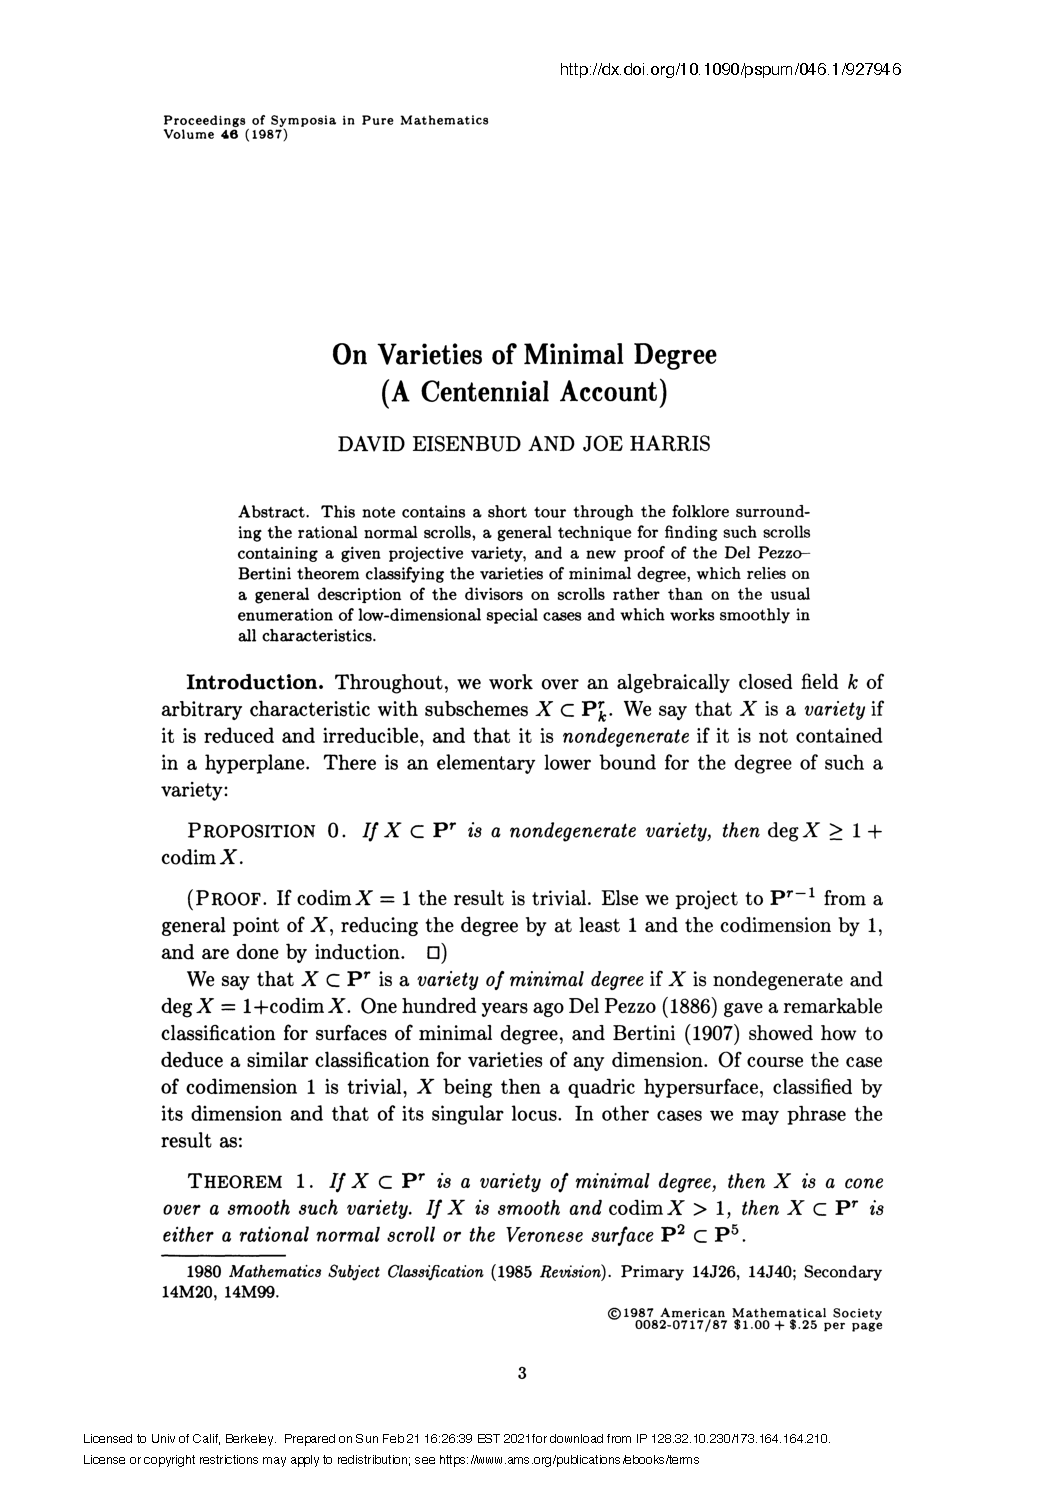
\includepdf[pages=1-11]{Centennial.pdf}

%footer for separate chapter files

\ifx\whole\undefined
%\makeatletter\def\@biblabel#1{#1]}\makeatother
\makeatletter \def\@biblabel#1{\ignorespaces} \makeatother
\bibliographystyle{msribib}
\bibliography{slag}

%%%% EXPLANATIONS:

% f and n
% some authors have all works collected at the end

\begingroup
%\catcode`\^\active
%if ^ is followed by 
% 1:  print f, gobble the following ^ and the next character
% 0:  print n, gobble the following ^
% any other letter: normal subscript
%\makeatletter
%\def^#1{\ifx1#1f\expandafter\@gobbletwo\else
%        \ifx0#1n\expandafter\expandafter\expandafter\@gobble
%        \else\sp{#1}\fi\fi}
%\makeatother
\let\moreadhoc\relax
\def\indexintro{%An author's cited works appear at the end of the
%author's entry; for conventions
%see the List of Citations on page~\pageref{loc}.  
%\smallbreak\noindent
%The letter `f' after a page number indicates a figure, `n' a footnote.
}
\printindex[gen]
\endgroup % end of \catcode
%requires makeindex
\end{document}
\else
\fi





